\makeatletter
\def\@makechapterhead#1{%
  \vspace*{5\p@}%
  {\parindent \z@ \centering \normalfont
    \ifnum \c@secnumdepth >\m@ne
      \if@mainmatter
        \Huge\bfseries %\@chapapp\space %\thechapter
	\vskip 4pt
        %\hrule height 2pt
        \par\nobreak
        \vskip 5\p@
      \fi
    \fi
    \interlinepenalty\@M
    \huge \bfseries #1\par\nobreak
\vskip 5pt

%\hrule height 2pt   
 \vskip 10\p@  
  }}
\makeatother
\chapter{anubaMdha - 1}

\lhead[\sl{anubaMdhagaLu}]{}
\rhead[]{\sl{anubaMdhagaLu}}

\begin{center}
{\Large koVSaTxkagaLu - \eng{Tables}}
\medskip

{\Large tUka matutx aLategaLu - \eng{Weights and Measures}}
\medskip

{\Large meTirxkf padadhxti - \eng{Metric System}}
\end{center}

\vskip .05cm

\begin{center}
{\large\bf darxvayxrAshiya aLate - \eng{Measure of mass}}
\end{center}

\begin{center}
\renewcommand{\arraystretch}{1.3}
\begin{tabular}{clcl}
$10$ & mili gArxM \eng{(mg)} & = & $1$ seMTigArxM\\
$10$ & seMTi gArxM \eng{(cg)} & = & $1$ Desi gArxM\\
$10$ & Desi gArxM \eng{(dg)} & = & $1$ gArxM\\
$10$ & gArxM \eng{(g)} & = & $1$ DekA gArxM\\
$10$ & DekA gArxM \eng{(dag)} & = & $1$ hekoTxV gArxM\\
$10$ & hekoTxV gArxM \eng{(kg)} & = & $1$ miriyA gArxM\\
$10$ & miriyA gArxM & = & $1$ kivxMTAlf\\
$10$ & kivxMTAlf & = & $1$ meTirxkf Tanf
\end{tabular}
\end{center}

\bigskip

\begin{center}
{\large\bf udadxLate  - \eng{Measure of length}}
\end{center}

\begin{center}
\renewcommand{\arraystretch}{1.3}
\begin{tabular}{clcl}
$10$ & mili miVTaru \eng{(mm)} & = & $1$ seMTi miVTaru\\
$10$ & seMTi miVTaru \eng{(cm)} & = & $1$ Desi miVTaru\\
$10$ & Desi miVTaru \eng{(dm)} & = & $1$ miVTaru\\
$10$ & miVTaru \eng{(m)} & = & $1$ DekA miVTaru\\
$10$ & DekA miVTaru \eng{(dam)} & = & $1$ hekoTxV miVTaru\\
$10$ & hekoTxV miVTaru \eng{(hm)} & = & $1$ kiloV miVTaru\\
$10$ & kiloV miVTaru \eng{(km)} & = & $1$ miriyA miVTaru
\end{tabular}
\end{center}

\newpage

\begin{center}
{\large\bf visitxVNaRda aLate  - \eng{Measure of Area}}
\end{center}

\begin{center}
\renewcommand{\arraystretch}{1.3}
\begin{tabular}{clcl}
$100$ & cadara mili miVTaru \eng{(sq mm)} & = & $1$ cadara seMTi miVTaru\\
$100$ & cadara seMTi miVTaru \eng{(sq cm)} & = & $1$ cadara Desi miVTaru\\
$100$ & cadara Desi miVTaru \eng{(sq dm)} & = & $1$ cadara miVTaru\\
$100$ & cadara miVTaru \eng{(sq m)} & = & $1$ cadara DekA miVTaru\\
$100$ & cadara DekA miVTaru \eng{(sq dam)} & = & $1$ cadara hekoTxV miVTaru\\
$100$ & cadara hekoTxV miVTaru \eng{(sq hm)} & = & $1$ cadara kiloV miVTaru\\
$100$ & cadara kiloV miVTaru \eng{(sq km)} & = & $1$ cadara miriyA miVTaru
\end{tabular}
\end{center}

\bigskip

\begin{center}
{\large\bf Gana aLate  - \eng{Measure of volume}}
\end{center}

\begin{center}
\renewcommand{\arraystretch}{1.3}
\begin{tabular}{clcl}
$1000$ & Gana mili miVTaru \eng{(cu mm)} & = & $1$ Gana seMTi miVTaru\\
$1000$ & Gana seMTi miVTaru \eng{(cu cm)} & = & $1$ Gana Desi miVTaru\\
$1000$ & Gana Desi miVTaru \eng{(cu dm)} & = & $1$ Gana miVTaru\\
$1000$ & Gana miVTaru \eng{(cu m)} & = & $1$ Gana DekA miVTaru\\
$1000$ & Gana DekA miVTaru \eng{(cu dam)} & = & $1$ Gana hekoTxV miVTaru\\
$1000$ & Gana hekoTxV miVTaru \eng{(cu hm)} & = & $1$ Gana kiloV miVTaru\\
$1000$ & Gana kiloV miVTaru \eng{(cu km)} & = & $1$ Gana miriyA miVTaru
\end{tabular}
\end{center}

\bigskip

\begin{center}
{\large\bf darxvada aLate  - \eng{Measure of fluid}}
\end{center}

\begin{center}
\renewcommand{\arraystretch}{1.3}
\begin{tabular}{clcl}
$10$ & mili liVTaru \eng{(ml)} & = & $1$ seMTi liVTaru\\
$10$ & seMTi liVTaru \eng{(cl)} & = & $1$ Desi liVTaru\\
$10$ & Desi liVTaru \eng{(dl)} & = & $1$ liVTaru\\
$10$ & liVTaru \eng{(l)} & = & $1$ DekA liVTaru\\
$10$ & DekA liVTaru \eng{(dal)} & = & $1$ hekoTxV liVTaru\\
$10$ & hekoTxV liVTaru \eng{(hl)} & = & $1$ kiloV liVTaru
\end{tabular}
\end{center}

\newpage

\begin{center}
{\large\bf meTirxkf padadhxtiyalilx pUvaRparxtayxyagaLu}
\medskip

\renewcommand{\arraystretch}{1.2}
\begin{tabular}{lllll}
\multicolumn{3}{l}{\bf pUvarxparxtayxya} & {\bf athaR} & {\bf guNaka}\\
\eng{Tera} & Tera & \eng{T} & $1$ Tirxliyanf & $10^{12}$\\
\eng{Giga} & giga & \eng{G} & $1$ biliyanf & $10^{9}$\\
\eng{Mega} & mega & \eng{M} & $1$ miliyanf & $10^{6}$\\
\eng{Kilo} & kiloV & \eng{K} & $1$ sAvira & $10^{3}$\\
\eng{Hecto} & hekoTxV & \eng{h} & $1$ nUru & $10^{2}$\\
\eng{Deca} & DekA & \eng{da} & hatutx & $10^{1}$\\
\eng{Deci} & Desi & \eng{d} & hatatxneV oMdu & $10^{-1}$\\
\eng{Centi} & seMTi & \eng{C} & nUraneV oMdu & $10^{-2}$\\
\eng{Milli} & mili & \eng{m} & sAviradalilx oMdu BAga & $10^{-3}$\\
\eng{Micro} & meYkorx & $\mu$ & miliyaninxna oMdu BAga & $10^{-6}$\\
\eng{Nano} & nAyxno & \eng{n} & biliyaninxnalilx oMdu BAga & $10^{-9}$\\
\eng{Pico} & peYko & \eng{P} & Tirxliyaninxnalilx oMdu BAga & $10^{-12}$ 
\end{tabular}
\end{center}

\bigskip

\begin{center}
{\large\bf kAgadada aLate - \eng{Paper Measure}}
\medskip

\renewcommand{\arraystretch}{1.2}
\begin{tabular}{l}
$24$ hALe = $1$ dasutx \eng{Quire}, $20$ dasutxgaLu = $1$ riVmu \eng{Ream}\\
$21\frac{1}{2}$ dasutx = $1$ mudarxkara riVmu ($516$ hALe) \eng{Printers Ream}\\
$2$ riVmu = $1$ baMDalu $1$ \eng{Bundle}\\
$10$ riVmu = $1$ beVlu $1$ \eng{Bale}
\end{tabular}
\end{center}

\bigskip

\begin{center}
{\large\bf meVlemxY aLate - \eng{Measure of Surface}}
\medskip

\renewcommand{\arraystretch}{1.2}
\begin{tabular}{clcl}
$10$ & miliyeVrfgaLu & = & $1$ seMTiyeVrf\\
$10$ & seMTiyeVrfgaLu & = & $1$ DesiyeVrf\\
$10$ & DesiyeVrfgaLu & = & $1$ Erf ($100$ ca.miV)\\
$10$ & ErfgaLu & = & $1$ DekeVrf\\
$10$ & DekeVrfgaLu & = & $1$ hekeTxVrf\\
$10$ & hekeTxVrfgaLu & = & $1$ kiloyeVrf\\
$100$ & hekeTxVrfgaLu & = & $1$ cadara kilomiVTarf
\end{tabular}
\end{center}

\bigskip

\begin{center}
{\large\bf saMKeyxgaLu - \eng{Numbers}}
\medskip

\renewcommand{\arraystretch}{1.2}
\begin{tabular}{ccc}
\eng{Roman}&\eng{Arabic}&\eng{Kannada}\\
roVmanf & arAyxbikf & kananxDa\\
\eng{I} & $1$ & 1\\
\eng{II} & $2$ & 2\\
\eng{III} & $3$ & 3\\
\eng{IV} & $4$ & 4\\
\eng{V} & $5$ & 5\\
\eng{VI} & $6$ & 6\\
\eng{VII} & $7$ & 7\\
\eng{VIII} & $8$ & 8\\
\eng{IX} & $9$ & 9\\
\eng{X} & $10$ & 10
\end{tabular}
\end{center}

\bigskip

\begin{center}
{\large\bf pusatxkagaLa aLate (aMgulagaLalilx) - \eng{Size of Books (in inches)}}
\bigskip

\renewcommand{\arraystretch}{1.3}
\begin{tabular}{lll}
\eng{Foolscap} & PUlfsxkAyxpf aSaTxdaLa & $6\dfrac{3}{4}\times 4\dfrac{1}{4}$\\[10pt]
\eng{Single Crown} & kwrxnf aSaTxdaLa & $7\dfrac{1}{2}\times 5$\\[10pt]
\eng{Demy} & Demi aSaTxdaLa & $8\dfrac{3}{8}\times 5\dfrac{5}{8}$\\[10pt]
\eng{Royal} & rAyalf aSaTxdaLa & $10\times 6\dfrac{1}{4}$\\[10pt]
\eng{Double Crown} & kwrxnf PoVliyo & $15\times 10$\\[5pt]
\eng{Royal Folio} & rAyalf PoVliyo & $20\times 12\dfrac{1}{2}$
\end{tabular}
\end{center}

\newpage

\begin{center}
{\large\bf kAlda aLate - \eng{Measure of Time}}
\medskip

\renewcommand{\arraystretch}{1.05}
\begin{longtable}{rlcll}
$60$ & sekeMDu & = & $1$ nimiSa & \eng{$1$ Minute}\\[3pt]
$60$ & nimiSa  & = & $1$ gaMTe & \eng{$1$ Hour}\\[3pt]
$24$ & gaMTe   & = & $1$ dina & \eng{$1$ Day}\\[3pt]
$7$  & dina    & = & $1$ vAra & \eng{$1$ Week}\\[3pt]
$15$ & dina    & = & $1$ pakaSx & \eng{$1$ Fortnight}\\[3pt]
$4$  & vAra    & = & $1$ tiMgaLu & \eng{$1$ Month}\\[3pt]
$12$ & tiMgaLu & = & $1$ vaSaR   & \eng{$1$ Year}\\[3pt]
$52$ & vAra    & = & $1$ vaSaR   & \eng{$1$ Year}\\[3pt]
$365$ & dina   & = & $1$ vaSaR   & \eng{$1$ Year}\\[3pt]
$366$ & dina   & = & $1$ adhika vaSaR & \eng{$1$ Leap year}\\[3pt]
$10$  & vaSaR  & = & $1$ dashamAna & \eng{$1$ Decade}\\[3pt]
$100$ & vaSaR  & = & $1$ shatamAna & \eng{$1$ Century}
\end{longtable}
\end{center}


%\medskip
%\begin{center}
%\begin{minipage}[c]{10cm}
%\begin{description}
%\item[sUcane~:] koVSaTxkada modalaneya aDaDx matutx kaMba sAlina saMKeyxgaLanunx kUDalu matutx kaLeyalu upayoVgisabeVku.

%\item[udA~:] saMkalana: $4+6=10$: vayxvakalana: $10-6=4$, $10-4=6$
%\end{description}
%\end{minipage}
%\end{center}

%\medskip
%\begin{center}
%\begin{minipage}[c]{10cm}
%\begin{description}
%\item[sUcane~:] koVSaTxkada modalaneya aDaDx matutx kaMba sAlina saMKeyxgaLanunx guNisalu matutx BAgisalu upayoVgisabeVku.

%\item[udA~:] guNAkAra : $8\times 6=48$ 

%~BAgAkAra : $48\div 6 = 8$

%~\phantom{iAAAAA} $48\div 8 = 6$
%\end{description}
%\end{minipage}
%\end{center}

\vskip .1cm

\begin{center}
{\bf\huge anubaMdha - 2}
\end{center}

\begin{center}
{\large\bf aMkegaLa sAthxna bele hesarugaLanunx sUcisuva paTiTx}

\smallskip
{\large\bf \eng{Table indicating the place value of Numbers}}
\end{center}

\begin{center}
\renewcommand{\arraystretch}{1.2}
\tabcolsep=4pt
\begin{tabular}{|c|c|c|c|c|c|c|c|}
\hline
 & & & (Eka) & & & & \\[-3pt]
sAvira & nUru & hatutx & biDi & dashamAMsha & dashAMsha & shatAMsha & sahasArxMsha\\[-3pt]
 & & & & biMdu & & & \\[10pt]
\rotatebox{90}{\eng{Thousands}} & \rotatebox{90}{\eng{Hundreds}} & \rotatebox{90}{\eng{Tens}} & \rotatebox{90}{\eng{Ones (Unit)}} & \rotatebox{90}{\eng{Decimal Point}} & \rotatebox{90}{\eng{Tenths}} & \rotatebox{90}{\eng{Hundredths}} & \rotatebox{90}{\eng{Thousandths}}\\
\hline
$1000$ & $100$ & $10$ & $1$ & $\leftarrow\quad \rightarrow$ & $\frac{1}{10}$ & $\frac{1}{100}$ & $\frac{1}{1000}$\\[5pt]
\hline
\end{tabular}
\end{center}

\begin{center}
\renewcommand{\arraystretch}{1.4}
\begin{tabular}{crll}
$\leftarrow\quad\rightarrow$ & \multicolumn{3}{p{8cm}}{biDisAthxnadiMda eDaBAgakekx parxtisAthxnadiMda inonxMdu sAthxnakekx hoVdaMtelAlx aMkegaLa sAthxna beleyu hatatxraSuTx hecucxtAtx hoVgutatxde.}\\[4pt]
& \multicolumn{3}{p{8cm}}{biDisAthxnadiMda balaBAgakekx parxtisAthxnadiMda inonxMdu sAthxnakekx hoVdaMtelAlx aMkegaLa sAthxna beleyu hatatxraSuTx kaDimeyAgutAtx hoVgutatxde.}\\
$10^{5}$ & $1,00,000$ & lakaSx & \eng{Lakh}\\
$10^{6}$ & $10,00,000$ & dashalakaSx & \eng{Million}\\
$10^{7}$ & $10,000,000$ & koVTi & \eng{Crore (10 Million)}\\
$10^{9}$ & $1,000,000,000$ & shata koVTi & \eng{Billion}\\
$10^{12}$ & $1,000,000,000,000$ & lakaSx koVTi & \eng{Trillion}
\end{tabular}
\end{center}

\vskip .8cm

\begin{center}
{\bf\huge anubaMdha - 3}
\end{center}

\begin{center}
{\large\bf sUtarxgaLu matutx niyamagaLu}

\smallskip
{\large\bf \eng{Formulae and Laws}}

\smallskip
{\large\bf lABa matutx naSaTx \ \ \eng{Profit and Loss}}
\end{center}

\begin{center}
\begin{tabular}{l@{\qquad}l}
lABa = mArida bele $-$ asalu & \eng{Profit = Selling price $-$ Cost price}\\[4pt]
naSaTx = asalu $-$ mArida bele & \eng{Loss = Cost price $-$ Selling price}
\end{tabular}
\end{center}

\vskip .3cm
\begin{center}
{\large\bf saraLa baDiDx \ \ \eng{Simple Interest}}
\end{center}

{\renewcommand{\arraystretch}{2.5}
\begin{longtable}{l@{\qquad\qquad}l}
saraLa baDiDx $=\dfrac{\text{asalu~} \times \text{~kAla~} \times \text{dara}}{100}$ & \eng{S.I.} = $\dfrac{\text{\eng{Ptr}}}{100}$\\
\multicolumn{2}{l}{\eng{Simple Interest} = $\dfrac{\text{\eng{Principal}} \times \text{\eng{time}} \times \text{\eng{rate}}}{100}$}\\
asalu $=\dfrac{100\times \text{baDiDx}}{\text{kAla} \times \text{dara}}$ & $\text{\eng{P}} = \dfrac{100~\text{\eng{I}}}{\text{\eng{t r}}}$\\
kAla = $\dfrac{100\times \text{baDiDx}}{\text{asalu}\times \text{dara}}$ & \eng{t} = $\dfrac{100~\text{\eng{I}}}{\text{\eng{P~r}}}$\\
dara = $\dfrac{100\times \text{baDiDx}}{\text{asalu} \times \text{kAla}}$ & \eng{r} = $\dfrac{100~\text{\eng{I}}}{\text{\eng{P~t}}}$\\[-.3cm]
\multicolumn{2}{l}{motatx = asalu $+$ saraLa baDiDx; \eng{Amount = Principal + Simple Interest}}\\[-.5cm]
\multicolumn{1}{l}{\eng{A = P + S.I.}}
\end{longtable}}

\vskip .3cm
\begin{center}
{\large\bf cakarx baDiDx \ \ \eng{Compound Interest}}
\end{center}
$$
\text{motatx = asalu} \left( 1+ \dfrac{\text{dara}}{100}\right)^{\text{kAla}};\qquad \text{\eng{A = P}} \left(1+\dfrac{\text{\eng{r}}}{100}\right)^{\text{\eng{n}}}
$$
cakarx baDiDx = motatx $-$ asalu
\smallskip

\noindent
\eng{Compound Interest} = \eng{Amount $-$ Principal}

\vskip .5cm
\begin{center}
{\large\bf gaNagaLu \ \ \text{\eng{Sets}}}
\end{center}

\noindent
$A$, $B$ matutx $C$ mUru gaNagaLAdAga,
\begin{itemize}
\item[\eng{(i)}] saMyoVga parivataRniVya niyama \ : \ $A\cup B = B \cup A$

\item[\eng{(ii)}] CeVdana parivataRniVya niyama \ : \ $A\cap B = B\cap A$

\item[\eng{(iii)}] saMyoVga sahavataRniVya niyama~:
$$
(A\cup B)\cup C=A\cup (B\cup C)
$$

\item[\eng{(iv)}] CeVdana sahavataRniVya niyama~:
$$
(A\cap B)\cap C=A\cap (B\cap C)
$$

\item[\eng{(v)}] viBAjaka niyama~:
\begin{align*}
& A\cup (B\cap C)=(A\cup B)\cap (A\cup C)\\[2pt]
& A\cap (B\cup C)=(A\cap B)\cup (A\cap C)\\[2pt]
& n(A\cup B)=n(A)+n(B)-n(A\cap B)
\end{align*}
$A\cup A'=\bigcup$, $A\cap A'=\phi$ $A'$ dare $A$ nunx $A$ ya pUrakagaNa enunxtAtxre.

$\bigcup$ = vishavxgaNa, \ $\phi=$ shUnayxgaNa.
\end{itemize}

\vskip .4cm
\begin{center}
{\large\bf karxmayoVjane, vikalapx, saMBavaniVyate}
\smallskip

{\large\bf \eng{Permutation, Combination, Probability}}
\end{center}

gaNAMsha $A$ yanunx $m$ vidhagaLalilx ArisabahudAgidudx matutx iMtaha parxtiyoMdu Ayekxya anaMtara gaNAMsha $B$ yanunx $n$ vidhagaLalilx ArisabahudAdare yugamx $(A,B)$ yanunx $mn$ vidhagaLalilx Arisabahudu. ideV niyamavanunx eraDakikxMta hecicxna saMdaBaRgaLigU upayoVgisabahudu.
\begin{center}
\renewcommand{\arraystretch}{1.5}
\begin{tabular}{l@{\qquad}l@{\qquad}l}
\multicolumn{3}{l}{${}_{n}P_{r} = n(n-1)(n-2)\ldots (n-r+1)$}\\
$_{n}P_{r}=\dfrac{\phase{n}}{\phase{n-r}}$ & $_{n}C_{r}=\dfrac{_{n}P_{r}}{\phase{r}}$ & $_{n}C_{r}=\dfrac{\phase{n}}{\phase{n-r}\cdot\phase{r}}$\\
$_{n}P_{r}={}_{n}C_{n-r}$ & $_{n}P_{1}=n$ & ${}_{n}P_{n}=\phase{n}$\\
$_{n}C_{1}=n$ & $\phase{O}=1$ & ${}_{n}C_{0}=1$\\
$_{n}C_{n}=1$ & &
\end{tabular}
\end{center}
GaTane $A$ ya saMBavaniVyate = $\dfrac{A~\text{upagaNadalilxruva PalitAMshagaLa saMKeyx}}{S~\text{nalilxruva PalitAMshagaLa saMKeyx}}$
\smallskip

\noindent
$\therefore~ P(A)=\dfrac{n(A)}{n(S)}$
\smallskip

\smallskip
\noindent
$P(A)+P(A')=1$, $A$ ya pUraka GaTane $A'$.


\vskip .5cm
\begin{center}
{\bf kaMtina vAyxpAra \ \ \eng{Instalment Buying}}
\end{center}
\begin{align*}
r &= \dfrac{2400 E}{n[(n+1)-2E]}\\[6pt]
r &= \frac{2400[np-B.A.]}{n\left[(n+1)p-2[np-B.A.]\right]}\\[6pt]
P &= \frac{2C[1200+r_{n}]}{n[2400+r(n-I)]}
\end{align*}

\newpage

\begin{tabular}{rcl}
ililx\qquad $r$ & = & dara\\[3pt]
$E$ &=& hecicxge haNa; \eng{Extra amount}\\[3pt] 
$n$ & = & kaMtugaLa saMKeyx; \eng{No. of instalments}\\[3pt]
$p$ & = & parxtiyoMdu tiMgaLa kaMtina haNa;\\[2pt]
    &   & \eng{Amount of each instalment}\\[3pt]
$B.A.$ & = & bAki uLidiruva haNa; \eng{Balance amount}\\[3pt]
$C$    & = & asalu bele; \eng{Cost price}
\end{tabular}

\vskip .5cm

\begin{center}
{\Large\bf vAyxpArada vayxvahAragaLu \ \ \eng{Accountancy}}
\medskip

{\large\bf veYyakitxka KAte \ \ \eng{Personal Account}}
\end{center}

\begin{itemize}
\item[\eng{(a)}] koTaTxvara KAteyalilx jamA viBAgadalilx dAKalisuvudu

\item[\eng{(b)}] paDedavara KAteyalilx KacuR viBAgadalilx dAKalisuvudu
\end{itemize}

\begin{center}
{\large\bf AsitxgaLu \ \ \eng{Real Account}}
\end{center}

\begin{itemize}
\item[\eng{(a)}] baMdadadxnunx KacuR viBAgadalilx dAKalisuvudu

\item[\eng{(b)}] koTaTxdadxnunx jamA viBAgadalilx dAKalisuvudu
\end{itemize}

\begin{center}
{\large\bf hesarina KAte \ \ \eng{Nominal Account}}
\end{center}

\begin{itemize}
\item[\eng{(a)}] KacuR naSaTxgaLanunx KacuR viBAgadalilx dAKalisuvudu

\item[\eng{(b)}] lABa AdAyagaLanunx jamA viBAgadalilx dAKalisuvudu
\end{itemize}

\begin{center}
{\large\bf aMkiaMshagaLu (saMKAyxkalanashAsatxrX) \ \ \eng{Statistics}}
\end{center}

sarAsari \eng{Mean} $\overline{X}$ = $\dfrac{\text{elAlx parimANagaLa motatx}}{\text{parimANagaLa saMKeyx}}$
\medskip

$\overline{X}=\dfrac{\Sigma x}{N}$ \ \ (vagiRVkarisada parimANagaLu)
\medskip

$\overline{X}=\dfrac{\Sigma fx}{N}$ \ \ (vagiRVkarisida parimANagaLu)

\smallskip
nijavAda rUDhi bele = $3\times $ mAdhayxma bele $-2 \, \times$ sarAsari bele

\smallskip
\eng{True mode = 3 $\times$ Median $-2\,\times$ Mean}
\smallskip

vagARMtarada madhayxbiMdu~:
\begin{gather*}
=\dfrac{\text{vagARMtarada keLagina miti + vagARMtarada meVlina miti}}{2}\\[5pt]
\text{\eng{Mid point of the C.L.}} = \dfrac{\text{\eng{Lower limit of C.I. + Upper limit of C.I.}}}{2}\\[3pt]
M=M' + \dfrac{\Sigma fd'}{N} \times C
\end{gather*}

\begin{tabular}{rcl}
ililx\qquad $M$ & = & nijavAda sarAsari\\[3pt]
            $M'$ & = & Uhisida sarAsari\\[3pt]
            $f$  & = & AvataR saMKeyx\\[3pt]
            $d'$ & = & $M'$ niMda Aguva GaTaka vicalane\\[3pt]
            $C$  & = & vagARMtarada gAtarx\\[3pt]
            $N$  & = & oTuTx parimANagaLa saMKeyx\\[3pt]
\multicolumn{3}{l}{\qquad vAyxpitx \eng{(Rangle)} = gariSaThx pArxpAtxMka $-$ kaniSaThx pArxpAtxMka}\\[3pt]
$R$ & = & $H-L$
\end{tabular}

\smallskip
vAyxpitxya vicalana guNAMka \eng{(Coefficient of Range)} = $\dfrac{H-L}{H+L}$
\medskip

madhayxda catuthaRka vAyxpitx \eng{(Inter Quartile Range)} =

\smallskip
= mUraneya catuthaRka bele $-$ modalaneya catuthaRka bele $=Q_{3}-Q_{1}$

\smallskip
catuthaRka vicalane \eng{Quartile deviation (Q.D.)} $=\dfrac{Q_{3}-Q_{1}}{2}$
\begin{align*}
Q_{1} &= L +\dfrac{\left(\frac{N}{4}-F\right)}{f_{m}}\times C\\[3pt]
Q_{2} &= L +\dfrac{\left(\frac{N}{2}-F\right)}{f_{m}}\times C\\[3pt]
Q_{3} &= L + \dfrac{\left(\frac{3N}{4}-F\right)}{f_{m}}\times C
\end{align*}

\begin{tabular}{rcp{7cm}<{\raggedright}}
ililx\qquad $L$ &=& madhayxma bele iruva vagARMtarada keLagina miti\\[3pt]
            $N$ &=& pArxpAtxMkagaLa saMKeyx\\[3pt]
            $F$ &=& madhayxma bele iruva vagARMtarada keLagaDe iruva AvaqtitxgaLa oTuTx saMcita motatx\\[3pt]
            $f_{m}$ &=& madhayxma bele iruva vagARMtarada Avaqtatx saMKeyx\\[3pt]
            $C$ &=& vagARMtarada gAtarx
\end{tabular}
$$
\left\{
\begin{array}{l}
\text{catuthaRka vicalane guNAMka}\\[2pt]
\text{\eng{(Coefficient of Quartile deviation)}}
\end{array}
\right\}=\dfrac{Q_{3}-Q_{1}}{Q_{3}+Q_{1}}
$$
\begin{center}
\begin{tabular}{c@{\qquad\qquad}c}
\begin{tabular}{l}
sarAsari vicalane\\[2pt]
\eng{Mean deviation}
\end{tabular}
$=\dfrac{\Sigma |d|}{N}$ &
\begin{tabular}{l}
sa.vi.\\[2pt]
\eng{M.D.}
\end{tabular}
$=\dfrac{\Sigma f|d|}{N}$\\[15pt]
(vagiRVkarisada saMKeyxgaLu) & (vagiRVkarisida saMKeyxgaLu)
\end{tabular}
\end{center}

\begin{tabular}{rl}
ililx $|d|$ = & cihenxgaLanunx nilaRkiSxsida $d$ ya shudadhx bele\\[3pt]
              & \eng{[Absolute value of $d$]} 
\end{tabular}

\vskip .5cm

\begin{center}
{\large\bf sarAsari vicalane guNAMka \ \ \eng{Coefficient of Mean deviation}}
\end{center}
\smallskip

madhayxma beleyiMda vicalateyanunx tegedukoMDAga.
\smallskip

sarAsari vicalane guNAMka $= \dfrac{\text{sarAsari vicalane}}{\text{madhayxma bele}}$

\smallskip
gaNita sarAsariyiMda vicalaneyanunx tegedukoMDAga

\smallskip
sarAsari vicalane guNAMka $=\dfrac{\text{sarAsari vicalane}}{\text{gaNita sarAsari}}$

\bigskip
\begin{center}
{\large\bf parxsaraNeya vicalane~ :~ \eng{Variance \boldmath$\sigma^{2}$}}
\end{center}

$\sigma^{2}=\dfrac{\Sigma d^{2}}{N}$ \ \ (vagiRVkarisada saMKeyxgaLu)

\medskip
$\sigma^{2}=\dfrac{\Sigma fd^{2}}{N}$ \ \ (vagiRVkarisida saMKeyxgaLu)

\newpage

\begin{center}
{\large\bf  mAnaka vicalane~ :~ \eng{Standard deviation : \boldmath$\sigma$}} 
\end{center}
\medskip

$\sigma = \sqrt{\dfrac{\Sigma d^{2}}{N}}$ \ \ (vagiRVkarisida saMKeyxgaLu)
\medskip

$\sigma = \sqrt{\dfrac{\Sigma fd^{2}}{N}}$ \ \ (vagiRVkarisida saMKeyxgaLu)

\medskip
\begin{tabular}{rl}
ililx\qquad $d$ & =~ sarAsari athavA madhayxkadiMda vicalane\\[3pt]
            $N$ & =~ parimANagaLa oTuTx saMKeyx; $f=$ AvataR saMKeyx
\end{tabular}

\smallskip
mApiRna guNAMka (vicaraNeya guNAMka) \eng{(Coefficient of variation)}
$$
=\dfrac{\sigma}{\overline{X}}\times 100
$$

ililx $\sigma=$ mAnaka vicalane; \ $\overline{X}=$ sarAsari

\bigskip

\begin{center}
{\large\bf savxyaM gaNa saMbaMdhagaLa bagegaLu - \eng{Types of relation in a set}}
\end{center}

\begin{itemize}
\item[\eng{(1)}] ananayxtA saMbaMdha \ \eng{Identity Relation}

gaNa $A$ nalilx saMbaMdha \ $R=\{(x,y)/x=y, x\in A, y\in A\}$

\item[\eng{(2)}] samaSiTx saMbaMdha \ \eng{Universal Relation}

datatx gaNa $A$ nalilx saMbaMdha $R=\{A\times A\}$

\item[\eng{(3)}] parxtiPalana saMbaMdha \ \eng{Reflexive Relation}

gaNa $A$ nalilx $(x,x)\in R\forall x\in A$

\item[\eng{(4)}] samamitiya saMbaMdha \ \eng{Symmetric Relation}

gaNa $A$ nalilx $R$ eMba saMbaMdha $xRy\Rightarrow yRx$

\item[\eng{(5)}] saMkarxmaka saMbaMdha \ \eng{Transitive Relation}

gaNa $A$ nalilx $x\in A$, $y\in A$ Agidudx $xRy$ matutx $yRz$

AdAga $xRz$ Agiruva $R$ saMbaMdha

\item[\eng{(6)}] samAnatA saMbaMdha \ \eng{Equivalence Relation}

gaNa $A$ meVlina $R$ saMbaMdha I keLagina saMbaMdhagaLanunx hoMdirabeVku.
\begin{description}[font=\normalfont]
\item[\qquad\quad~~\eng{(i)}] parxtiPalana saMbaMdha

\item[\qquad\quad~\eng{(ii)}] samamitiya saMbaMdha

\item[matutx \ \ \eng{(iii)}] saMkarxmaka saMbaMdha
\end{description}
\end{itemize}

\smallskip
\begin{center}
{\large\bf sherxVDhi matutx sherxVNigaLu - \eng{Sequence and Series}}
\medskip

\renewcommand{\arraystretch}{1.2}
\begin{tabular}{|c|c|c|}
\hline
vidhagaLu & sherxVDhiya & sherxVNi\\
          & $n$ neya pada & (sherxVNiya $n$ padagaLa motatx)\\
\hline
samAMtara & \multirow{2}{*}{$T_{n}=[a+(n-1)d]$} & \multirow{2}{*}{$S_{n}=\dfrac{n}{2}(a+l)$}\\
\eng{Arthmetic} & &\\[7pt]
                & & $S_{n}=\dfrac{n}{2}[2a+(n-1)d]$\\[10pt]
guNoVtatxra & \multirow{2}{*}{$T_{n}=ar^{n-1}$} & \multirow{2}{*}{$S_{n}=a\left[\dfrac{(1-r^{n})}{(1-r)}\right]\quad (r<1)$}\\
\eng{Geometric} & & \\[10pt]
& & \multirow{2}{*}{$S_{n}=a\left[\dfrac{(r^{n}-1)}{(r-1)}\right]\quad (r>1)$}\\
 &&\\
\eng{Harmonic} & \multirow{2}{*}{$T_{n}=\dfrac{1}{[a+(n-1)d]}$}&\\[-3pt]
harAtamxka &  &\\[5pt]
\hline
\end{tabular}

\medskip
\begin{tabular}{rcl}
ililx\qquad $T_{n}$ & = & $n$ neV pada $(n=1,2,3\ldots)$\\
            $S_{n}$ & = & $n$ padagaLa motatx\\
            $a$    & = & modalane pada\\
            $d$    & = & sAmAnayx vayxtAyxsa\\
            $l$    & = & samAMtara sherxVDhiya $n$ neV pada\\
            $r$    & = & sAmAnayx anupAta
\end{tabular}
\end{center}

modalane $n$ sAvxBAvika saMKeyxgaLa motatx : $\Sigma n=\dfrac{n(n+1)}{2}$

\vskip .1cm

$a$, $b$ gaLu $(a>b)$ eraDu dhana saMKeyxgaLu. $A$, $G$ matutx $H$ gaLu karxmavAgi

$a$, $b$ gaLa naDuvina samAMtara, guNoVtatxra matutx harAtamxka mAdhayxgaLAdare
$$
A=\dfrac{a+b}{2}\quad G=\sqrt{ab}\quad H = \dfrac{2ab}{a+b}\quad G^{2}=AH
$$

\vskip .5cm
\begin{center}
{\large\bf cihenxgaLa niyama}
\end{center}
\smallskip

\begin{itemize}
\item[\eng{(i)}] saMkalana : \eng{Addition}

$(+)+(+)=+$

$(-)+(-)=-$

\smallskip
dhana matutx QuNa rAshigaLanunx kUDidAga motatxvu doDaDx rAshiya cihenxyanunx hoMdutatxve.

\item[\eng{(ii)}] guNAkAra : \eng{Multiplication}

$(+)\times (+)=+$

$(-)\times (-)=+$

$(+)\times (-)=-$

$(-)\times (+)=-$

\item[\eng{(iii)}] BAgAkAra~:

BAjaka) BAjayx (BAgalabadhx

\bigskip
\qquad\quad~$\overline{\underline{\text{~sheVSa~}}}$

\smallskip
BAjayx = BAjaka $\times$ BAgalabadhx + sheVSa

\eng{Dividend = Divisor $\times$ Quotient + Remainder}

\item[\eng{(iv)}] cwkaLi kAgadadalilx nideVRshAMkagaLa cihenxgaLu.

\medskip
\begin{tabular}{lccccc}
\eng{I} & neV & pAdadalilx & nideVRshAMkagaLa & cihenx & $(+,+)$\\[3pt]
\eng{II} & neV & '' & '' & '' & $(-,+)$\\[3pt]
\eng{III} & neV & '' & '' & '' & $(-,-)$\\[3pt]
\eng{IV}  & neV & '' & '' & '' & $(+,-)$
\end{tabular}
\begin{figure}[H]
\centering
\includegraphics{figures/app01.eps}
\end{figure}
\end{itemize}

\newpage

%\begin{center}
\centerline{\large\bf visatxraNe sUtarxgaLu. \eng{Expansion formulae}}
%\end{center}
\begin{align*}
& (x+a)(x+b)=x^{2}+(a+b)x+ab\\
& (a+b)(a-b)=a^{2}-b^{2}\\
& (x+a)(x+b)(x+c)=x^{3}+x^{2}(a+b+c)+\\
&\hspace{3.6cm} x(ab+bc+ca)+abc\\
& (a+b)^{2}=a^{2}+2ab+b^{2}\\
& (a-b)^{2}=a^{2}-2ab+b^{2}\\
& (a+b+c)^{2}=a^{2}+b^{2}+c^{2}+2ab+2bc+2ca\\
& (a+b)^{3}=a^{3}+3ab(a+b)+b^{3}\qquad\text{athavA}\\
& (a+b)^{3}=a^{3}+3a^{2}b+3ab^{2}+b^{3}\\
& (a-b)^{3}=a^{3}-3ab(a-b)-b^{3}\qquad\text{athavA}\\
& (a-b)^{3}=a^{3}-3a^{2}b+3ab^{2}-b^{3}\\
& (a+b+c)^{3}=a^{3}+b^{3}+c^{3}+3(a+b)(b+c)(c+a)\\
& (a-b)(b-c)(c-a)=a(b^{2}-c^{2})+b(c^{2}-a^{2})+c(a^{2}-b^{2})\\
& \Sigma a^{2}(b-c)=a^{2}(b-c)+b^{2}(c-a)+c^{2}(a-b)\\
& \Sigma a(b+c)=a(b+c)+b(c+a)+c(a+b)\\
& \Sigma ab=ab+bc+ca
\end{align*}
%\begin{center}
\centerline{\large\bf apavatiRsuva sUtarxgaLu : \eng{Factorisation formulae}}
%\end{center}
\begin{align*}
& x^{2}+x(a+b)+ab=(x+a)(x+b)\\
& a^{2}+2ab+b^{2}=(a+b)^{2}\\
& a^{2}-2ab+b^{2}=(a-b)^{2}\\
& a^{2}-b^{2}=(a+b)(a-b)\\
& x^{3}+x^{3}(a+b+c)+x(ab+bc+ca)+abc=\\
& \hspace{4cm} (x+a)(x+b)(x+c)\\
& a^{3}+3a^{2}b+3ab^{3}+b^{3}=(a+b)^{3}\\
& a^{3}-3a^{2}b+3ab^{2}-b^{3}=(a-b)^{3}\\
& a^{3}+b^{3}=(a+b)(a^{2}-ab+b^{2})\\
& a^{3}-b^{3}=(a-b)(a^{2}+ab+b^{2})\\
& a^{2}+b^{2}+c^{2}+2ab+2bc+2ca=(a+b+c)^{2}\\
& a^{2}(b-c)+b^{2}(c-a)+c^{2}(a-b)=-(a-b)(b-c)(c-a)\\
& a^{3}+b^{3}+c^{3}-3abc=(a+b+c)(a^{2}+b^{2}+c^{2}-ab-bc-ca)\\
&\qquad = \frac{1}{2}(a+b+c)[(a-b)^{2}+(b-c)^{2}+(c-a)^{2}]\\
&\qquad = (a+b+c)[(a+b+c)^{2}-3(ab+bc+ca)]\\
& a^{4}+a^{2}b^{2}+b^{4}=(a^{2}+ab+b^{2})(a^{2}-ab+b^{2})\\
& ab(a-b)+bc(b-c)+ca(c-a)=-(a-b)(b-c)(c-a)
\end{align*}
$(a+b)^{2}$ matutx $(a-b)^{2}$ gaLa naDuvina aMtara saMbaMdha
\begin{align*}
& (a+b)^{2}=(a-b)^{2}+4ab\\
& (a-b)^{2}=(a+b)^{2}-4ab\\
& (a+b)^{2}-(a-b)^{2}=4ab
\end{align*}

\vskip .5cm

\begin{center}
{\large\bf GAtagaLu matutx parxtiGAtagaLu niyamagaLu}
\smallskip

{\large\bf\eng{Law of Indices and Logarithms}}

\bigskip
\renewcommand{\arraystretch}{2}
\begin{tabular}{r@{\;\,}l@{\qquad}r@{\;\,}l@{\qquad}r@{\;\,}l}
\eng{(i)} & $a^{m}+a^{n}=a^{m+n}$ & \eng{(ii)} & $(a^{m})^{n}= a^{mn}$\\
\eng{(iii)} & \multicolumn{5}{l}{$\dfrac{a^{m}}{a^{n}}=a^{m-n}(m>n) \quad\dfrac{a^{m}}{a^{n}}=\dfrac{1}{a^{n-m}}$ ($n>m$ AgidAdxga)}\\[4pt]
\eng{(iv)} & $(ab)^{m}=a^{m}b^{m}$ & \eng{(v)} & $\left[\dfrac{a}{b}\right]^{m}=\dfrac{a^{m}}{b^{m}}$ & 
\eng{(vi)} & $a^{-m}=\dfrac{1}{a^{m}}$\\[4pt]
\eng{(vii)} & $\dfrac{1}{a^{-m}}=a^{m}$ & \eng{(viii)} & $a^{0}=1$ & & 
\end{tabular}
\end{center}
iciCxta saMKeyx $(n)$ yanunx paDeyalu A saMKeyxya AdhArAMka $(b)$ yanunx yAva GAta $(l)$ kekx ErisabeVkoV A GAtavanunx saMKeyxya laGugaNaka $(\log n)$ enunxtAtxre.
$$
\log_{b}n=l\Leftrightarrow b^{l}=n
$$
$b=n$ samiVkaraNavu $b$ AdhAra saMKeyxyuLaLx `$n$' matutx `$l$'ra saMbaMdhavanunx tiLisutatxde.

$\therefore~ b^{l}=n$ AdAga $l=\log_{b}n$ Agutatxde.
\begin{align*}
& \log_{b}(mn)=\log_{b}m+\log_{b}n\\
& \log_{b}\dfrac{m}{n}=\log_{b}m-\log_{b}n\\
& \log_{b}(m)^{p}=p\log_{b}m\\
& \log_{b} m = \dfrac{\log_{e}m}{\log_{e}b}
\end{align*}
ma.sA.a. matutx la.sA.a. \ \ \eng{H.C.F. and L.C.M.}
\begin{center}
\begin{tabular}{@{}l@{\qquad}l@{\qquad}l}
$A=$ oMdaneya biVjoVkitx & $B=$ eraDaneya biVjoVkitx & $H=$ ma.sA.a.\\[3pt]
$L=$ la.sA.a. AdAga & $A\times B=H\times L$ &
\end{tabular}
\end{center}
$$
A=\dfrac{H\times L}{B}\qquad B=\dfrac{H\times L}{A}\qquad H=\dfrac{A\times B}{L}\qquad L=\dfrac{A\times B}{H} 
$$


\begin{center}
{\large\bf vagaR samiVkaraNa \ \ \eng{Quadratic equation}}
\end{center}

AdashaRrUpa \eng{Standard form} $ax^{2}+bx+c=0$

\smallskip
$ax^{2}+bx+c=0$ AdAga samiVkaraNada mUlagaLu
$$
x=\dfrac{-b\pm \sqrt{b^{2}-4ac}}{2a}
$$

\smallskip
$m$ matutx $n$ gaLu $ax^{2}+bx+c=0$ na mUlagaLAdare

\smallskip
\smallskip
mUlagaLa motatx $=m+n=\dfrac{-b}{a}=\dfrac{-x\text{~ na sahApavataRna}}{x^{2}\text{~ na sahApavataRna}}$
\smallskip

mUlagaLa guNalabadhx $=mn=\dfrac{c}{a}=\dfrac{\text{sithxra saMKeyx}}{x^{2}\text{~ na sahApavataRna}}$
\smallskip

$m$ matutx $n$ gaLu vagaR samiVkaraNada mUlagaLAdare A vagaRsamiVkaraNa $x^{2}-(m+n)x+mn=0$ Agutatxde.

\smallskip
athavA $x^{2}-{}$ (mUlagaLa motatx) $x+{}$ mUlagaLa guNalabadhx $=0$.
\begin{center}
\renewcommand{\arraystretch}{1.2}
\begin{tabular}{|r@{\;\;}p{4cm}|r@{\;\;}p{4cm}<{\raggedright}|}
\multicolumn{2}{c}{shoVdhaka : \eng{DISCRIMINANT}} & \multicolumn{2}{c}{$\Delta = b^{2}-4ac$}\\
\hline
\multicolumn{2}{|c|}{shoVdhaka $\Delta$ da bele} & \multicolumn{2}{c|}{mUlagaLa savxBAva}\\
\hline
 & $\Delta > 0$ & & \\
\eng{(i)} & $\Delta$ oMdu pUNaR vagaR & \eng{(i)} & mUlagaLu vAsatxva matutx BAgalabadhx saMKeyxgaLu.\\
\eng{(ii)} & $\Delta$ oMdu pUNaR vagaRvalalx & \eng{(ii)} & mUlagaLu vAsatxva matutx aBAgalabadhx saMKeyxgaLu.\\
\hline
 & $\Delta = 0$ & & mUlagaLu neYja matutx sama\\
\hline
 & $\Delta < 0$ & & mUlagaLu saMkiVNaR saMKeyxgaLu\\
\hline
\end{tabular}
\end{center}

\vskip .5cm

\begin{center}
{\large\bf biVjagaNitada vAsatxvika saMKeyxgaLa niyama}
\smallskip

{\large\bf\eng{Laws of real numbers in Algebra}}
\end{center}

{\bf \boldmath$a$, $b$ matutx $c$ gaLu vAsatxvika saMKeyxgaLAdAga}
\begin{enumerate}
\renewcommand{\labelenumi}{\eng{\theenumi.}}
\item saMkalanada parivataRna niyama~:

\eng{Commutative property of addition :}

$\forall \ a,b,\in R$, \ \ $a+b=b+a$

\item guNAkArada parivataRna niyama :

\eng{Commutative property of multiplication :}

$\forall \ a,b,\in R$, \ \ $a\times b=b\times a$

\item saMkalanada sahavataRna niyama :

\eng{Associative property of addition :}

$\forall \ a,b,c,\in R$, \ \ $a+(b+c)=(a+b)+c$

\item guNAkArada sahavataRna niyama :

\eng{Associative property of Multiplication :}

$a\times (b\times c)=(a\times b)\times c$, \ \ $\forall \ a,b,c,\in R$

\item viBAjakada niyama :

\eng{Distributive property :}

$\forall \ a,b,c,\in R$,  \ \ $a(b+c)=ab+ac$, \ \ $(b+c)a=ba+ca$

\item saMkalanada ananayxtAMsha `$0$'

\eng{Identity element w.r.t. addition is `$0$'}

$\forall \ a\in R$, \ \ $a+0=0+a=a$

\item guNAkArada ananayxtAMsha $1$.

\eng{Identity element w.r.t. multiplication is $1$.}

$\forall \ a\in R$, \ \ $a\times 1= 1\times a=a$

\item saMkalanada parxtiloVma :

\eng{Additive Inverse :}

$\forall a\in R\exists - a\in R/(+a)+(-a)=(-a)+(+a)=0$ AdAga, 

$(-a)$ yanunx $(+a)$ ya saMkalanada parxtiloVma enunxtetxVve.

\item guNAkArada parxtiloVma :

\eng{Multiplicative Inverse :}

$\forall \ a\in R\exists \dfrac{1}{a}\in R/ a \times\dfrac{1}{a}=\dfrac{1}{a}\times a=1$ AdAga, 

$\dfrac{1}{a}$ yanunx $a$ ya guNAkAra parxtiloVma enunxtetxVve.
\end{enumerate}

\newpage

\begin{landscape}

\begin{center}
{\large\bf samataLAkaqtigaLa visitxVNaR matutx sutatxLateyanunx
 kaMDuhiDiyalu sUtarxgaLu}
\smallskip

{\large\bf \eng{Formulae to find the area and perimeter of plane figures}}
\end{center}

\begin{center}
%\tabcolsep=3pt
\renewcommand{\arraystretch}{1.1}
\begin{longtable}{|c|l|c|c|c|}
\hline
karxma & \multicolumn{1}{c|}{Akaqtiya hesaru} & visitxVNaR $A$ & sutatxLate $p$ & citarx\\[-2pt]
saMKeyx & \multicolumn{1}{c|}{\eng{Name of the}} & \eng{Area} & \eng{Perimeter} & \eng{Figure}\\[-2pt]
\eng{Sl.~No.} & \multicolumn{1}{c|}{\eng{figure}} & (cadara mAnagaLalilx) & (mAnagaLalilx) &\\
\hline
\eng{I} & \multicolumn{1}{c|}{\eng{II}} & \eng{III} & \multicolumn{1}{c}{\eng{IV}} & \eng{V}\\
\hline
 &&&\multicolumn{2}{c|}{}\\[-5pt]
\endfirsthead
\hline
\eng{I} & \multicolumn{1}{c|}{\eng{II}} & \eng{III} & \multicolumn{1}{c}{\eng{IV}} & \eng{V}\\
\hline
\endhead
\endfoot
\endlastfoot
$1$ & 
\begin{tabular}{l}
tirxBuja\\[3pt] 
\eng{Triangle}
\end{tabular} & $A=\dfrac{1}{2}bh$ & \multicolumn{2}{c|}{\begin{tabular}[c]{c}\includegraphics[scale=.9]{figures/app02.eps}\end{tabular}}\\
\hline
$2$ & 
\begin{tabular}{l}
samabAhu tirxBuja\\[3pt] 
\eng{Equilateral}\\[3pt]
\eng{triangle}
\end{tabular} &
$A=\dfrac{\sqrt{3}\times a^{2}}{4}$ & \multicolumn{1}{c}{\raisebox{.7cm}{$p=3a$}} & \begin{tabular}[c]{@{\kern -1.5cm}c@{}} \includegraphics[scale=.9]{figures/app03.eps} 
\end{tabular}\\ 
\hline
$3$ & 
\begin{tabular}{l}
viSamabAhu\\[3pt] 
tirxBuja\\[3pt]
\eng{Scalene}\\[3pt]
\eng{triangle}
\end{tabular} &
\begin{tabular}{l}
$A=\sqrt{s(s-a)(s-b)(s-c)}$\\[3pt]
ililx \ \ $s=\dfrac{a+b+c}{2}$
\end{tabular} &
\multicolumn{1}{c}{\raisebox{.7cm}{$p=a+b+c$}} & 
\begin{tabular}[c]{@{\kern -1cm}c}
\hfill\includegraphics[scale=.9]{figures/app04.eps}
\end{tabular}\\
\hline
$4$ & 
\begin{tabular}{l}
laMbakoVna\\
tirxBuja\\
\eng{Right angled}\\
\eng{triangle}
\end{tabular} &
$A=\dfrac{ab}{2}$ & 
\multicolumn{2}{c|}{
\begin{tabular}[c]{r}
$p=a+b+\sqrt{a^{2}+b^{2}}$\\[4pt]
\includegraphics[scale=.9]{figures/app05.eps}
\end{tabular}}\\
\hline
$5$ &
\begin{tabular}{l}
catuBuRja\\[3pt]
\eng{Quadrilateral}
\end{tabular} &
$A=\dfrac{1}{2}d(h_{1}+h_{2})$ &
\multicolumn{2}{c|}{
\begin{tabular}[c]{c}
\includegraphics[scale=.9]{figures/app04.eps}\\[4pt]
$AC=d$; $DE=h_{1}$; $BF=h_{2}$
\end{tabular}}\\
\hline
$6$ & 
\begin{tabular}{l}
samAnAMtara\\
catuBuRja\\
\eng{Parallelogram}
\end{tabular}
& 
$A=bh$ &
\multicolumn{2}{c|}{ 
\begin{tabular}[c]{r}
$p=2(a+b)$\qquad\qquad\qquad\\[3pt]
\includegraphics[scale=.9]{figures/app07.eps}
\end{tabular}}\\
\hline
$7$ & 
\begin{tabular}{l}
Ayata/Aya\\
\eng{Rectangle}
\end{tabular}
& 
$A=lb$ &
\multicolumn{2}{c|}{ 
\begin{tabular}[c]{r}
$p=2(l+b)$\qquad\qquad\qquad\\[4pt]
\includegraphics[scale=.9]{figures/app08.eps}
\end{tabular}}\\
\hline
$8$ & 
\begin{tabular}{l}
cwka, vagaR\\
\eng{Square}
\end{tabular}
& 
$A=a^{2}$ &
\multicolumn{2}{c|}{ 
\begin{tabular}[c]{r}
$p=4a$\qquad\qquad\qquad\\[4pt]
\includegraphics[scale=.9]{figures/app09.eps}
\end{tabular}}\\
\hline
$9$ & 
\begin{tabular}{l}
vajArxkaqti\\
\eng{Rhombus}
\end{tabular}
& 
$A=\dfrac{1}{2}d_{1}d_{2}$ &
\multicolumn{2}{c|}{ 
\begin{tabular}[c]{r}
$p=4a$\qquad\qquad\qquad\\[4pt]

\includegraphics[scale=.9]{figures/app10.eps}\\
\multicolumn{1}{c}{$AC=d_{1}$, $BD=d_{2}$}
\end{tabular}}\\
\hline
&&&\multicolumn{2}{c|}{}\\
$10$ & 
\begin{tabular}{l}
gALipaTa\\
\eng{Kite}
\end{tabular}
& 
$A=\dfrac{1}{2}d_{1}d_{2}$ &
\multicolumn{2}{c|}{ 
\begin{tabular}[c]{r}
\includegraphics[scale=.9]{figures/app10a.eps}~~~~~~~~~~~~~~~~~~\\
\multicolumn{1}{c}{$AB=AD$, $BC=DC$, $A=\frac{1}{2}\times d_{1}\times d_{2}$}
\end{tabular}}\\
\hline
\newpage
&&&\multicolumn{2}{c|}{}\\[-5pt]
$11$ & 
\begin{tabular}{l}
tArxpijayx\\
\eng{Trapezium}
\end{tabular}
& 
$A=\dfrac{1}{2}h(a+b)$ &
\multicolumn{2}{c|}{ 
\begin{tabular}[c]{c}
\includegraphics[scale=.9]{figures/app11.eps}\\
$DE=h$, $AB=a$, $DC=b$
\end{tabular}}\\
\hline
$12$ & 
\begin{tabular}{l}
samaSaDuBxja\\
\eng{Regular}\\
\eng{Hexagon}
\end{tabular}
& 
$A=\dfrac{\sqrt{3}\times a^{2}}{4}\times 6$ &
\multicolumn{2}{c|}{ 
\begin{tabular}[c]{r@{}}
$p=6a$\qquad\qquad\qquad\quad\,\\
\includegraphics[scale=.9]{figures/app12.eps}\\
\end{tabular}}\\
\hline
$13$ & 
\begin{tabular}{l}
vaqtatx\\
\eng{Circle}
\end{tabular}
& 
$A=\pi r^{2}$ &
\multicolumn{2}{c|}{ 
\begin{tabular}[c]{c}
$p=2\pi r$\\[1pt]
athavA\\[1pt]
$p=\pi d$\\[1pt]
\includegraphics[scale=.9]{figures/app13.eps}\\
\end{tabular}}\\
\hline
\end{longtable}
\end{center}

\begin{center}
{\large\bf niyata GanAkaqtigaLa meVlemxY visitxVNaR matutx gAtarxvanunx
 kaMDuhiDiyalu sUtarxgaLu}
\medskip

{\large\bf \eng{Formulae to find the surface area and volume of}
 \eng{regular solids}}

\smallskip

\renewcommand{\arraystretch}{1.1}
%\tabcolsep=5pt
\begin{longtable}{|c|l|c|c|c|c|}
\hline
karxma & \multicolumn{1}{c|}{Ganada hesaru} & Ore meVlemxY visitxNaR  & oTuTx meVlemxY & gAtarx & citarx Gana mAna\\[-1pt]
            &\multicolumn{1}{c|}{}  & ca. mAna &visitxNaR & Gana. mAna & \\[-1pt]
saMKeyx & \multicolumn{1}{c|}{\eng{Name of the}} & \eng{Lateral} & \eng{Total surface} & \eng{Volume} & \eng{Figure}\\[-1pt]
\eng{Sl.~No.} & \multicolumn{1}{c|}{\eng{Solid}} & \eng{surface area (L.S.A.)} & \eng{area (T.S.A.)} & \eng{V} &\\
\hline
\eng{I} & \multicolumn{1}{c|}{\eng{II}} & \eng{III} & \eng{IV} & \eng{V} & \eng{VI}\\
\hline
\endfirsthead
\hline
\eng{I} & \multicolumn{1}{c|}{\eng{II}} & \eng{III} & \eng{IV} & \eng{V} & \eng{VI}\\
\hline
\endhead
\hline
\endfoot
\hline
\endlastfoot
&&&&&\\[-3pt]
$1$ & 
\begin{tabular}{l}
tirxkoVna paTaTxka\\[3pt] 
\eng{Triangular}\\[3pt]
\eng{prism}
\end{tabular} & \eng{ph} & \eng{2B + ph} & \eng{Bh} & \begin{tabular}[c]{c}\includegraphics[scale=.9]{figures/app14.eps}\end{tabular}\\
\hline
&&&&&\\[-3pt]
$2$ & 
\begin{tabular}{l}
vagaR goVpura\\[3pt] 
\eng{Square}\\[3pt]
\eng{Pyramid}
\end{tabular} & $\dfrac{\text{\eng{p}}l}{2}$ & $\text{\eng{B}}+\dfrac{\text{\eng{p}}l}{2}$ & $\dfrac{\text{\eng{\eng{Bh}}}}{3}$ & \begin{tabular}[c]{c}\includegraphics[scale=.9]{figures/app15.eps}\end{tabular}\\
\hline
$3$ & 
\begin{tabular}{l}
laMba vaqtitxVya\\[3pt] 
siliMDarf\\[3pt]
\eng{Right circular}\\[3pt]
\eng{cylinder}
\end{tabular} & $2\pi\eng~rh$ & $2\pi r(r+h)$ & $\pi r^{2}h$ & \begin{tabular}[c]{c}\includegraphics[scale=.9]{figures/app16.eps}\end{tabular}\\
\hline
$4$ & 
\begin{tabular}{l}
laMbavaqtitxVya\\[3pt]
shaMku\\[3pt] 
\eng{Right Circular}\\[3pt]
\eng{cone}
\end{tabular} & $\pi rl$ & $\pi r(r+l)$ & $\dfrac{\pi r^{2}h}{3}$ & \begin{tabular}[c]{c}\includegraphics[scale=.9]{figures/app17.eps}\end{tabular}\\
\hline
&&&&&\\[-5pt]
$5$ & 
\begin{tabular}{l}
goVLa\\[3pt] 
\eng{Sphere}\\
\end{tabular} & - & $4\pi r^{2}$ & $\dfrac{4}{3}\pi r^{3}$ & \begin{tabular}[c]{c}
\includegraphics[scale=.9]{figures/app18.eps}\end{tabular}\\
\hline
$6$ & 
\begin{tabular}{l}
ToLuLx\\[3pt]
adhaR goVLa\\[3pt]
\eng{Hollow Hemi}\\[3pt]
\eng{Sphere}
\end{tabular} & - & $2\pi r^{2}$ & $\dfrac{2}{3}\pi r^{3}$ & \begin{tabular}[c]{c}
\includegraphics[scale=.9]{figures/app19.eps}\end{tabular}\\
\hline
$7$ & 
\begin{tabular}{l}
gaTiTx\\[3pt]
adhaR goVLa\\[3pt]
\eng{Solid Hemi}\\[3pt]
\eng{Sphere}
\end{tabular} & - & $3\pi r^{2}$ & $\dfrac{2}{3}\pi r^{3}$ & \begin{tabular}[c]{c}
\includegraphics[scale=.9]{figures/app20.eps}\end{tabular}\\
\hline
&&&&&\\[-5pt]
$8$ & 
\begin{tabular}{l}
Ayata Gana\\[3pt]
\eng{Cuboid}
\end{tabular} & $2h(l+b)$ & $2(lb+bh+lh)$ & $l\times b\times h$ & \begin{tabular}[c]{c}\includegraphics[scale=.9]{figures/app21.eps}\end{tabular}\\
\hline
&&&&&\\[-5pt]
$9$ & 
\begin{tabular}{l}
Gana\\[3pt]
\eng{Cube}
\end{tabular} & $4l^{2}$ & $6l^{2}$ & $l^{3}$ & \begin{tabular}[c]{c}\includegraphics[scale=.9]{figures/app22.eps}\end{tabular}\\
\hline
\end{longtable}
\end{center}
\end{landscape}

\vskip .5cm
\begin{center}
{\large\bf \eng{Pascal's Triangle} \ \ pAsakxlana tirxBuja}
\end{center}
\begin{gather*}
1\\
1 \qquad 1\\
1\qquad 2\qquad 1\\
1\qquad 3\qquad 3\qquad 1\\
1\qquad 4\qquad 6\qquad 4\qquad 1
\end{gather*}

\vskip .5cm

\begin{center}
{\large\bf tirxBujAkArada saMKeyxgaLu}
\medskip

{\large\bf \eng{Triangular Numbers}}
\bigskip

\begin{tabular}{c@{\qquad}r}
$\bullet$ & $1$\\[3pt]
$\bullet$\qquad $\bullet$ & $3$\\[3pt]
$\bullet$\qquad $\bullet$\qquad $\bullet$ & $6$\\[3pt]
$\bullet$\qquad $\bullet$\qquad $\bullet$\qquad $\bullet$ & $10$\\[3pt]
$\bullet$\qquad $\bullet$\qquad $\bullet$\qquad $\bullet$\qquad $\bullet$ & $15$\\[3pt]
$\bullet$\qquad $\bullet$\qquad $\bullet$\qquad $\bullet$\qquad $\bullet$\qquad $\bullet$ & $21$\\[3pt]
$\bullet$\qquad $\bullet$\qquad $\bullet$\qquad $\bullet$\qquad $\bullet$\qquad $\bullet$\qquad $\bullet$ & $28$
\end{tabular}
\end{center}

\vskip .7cm

\begin{center}
{\huge\bf anubaMdha - 4}
\bigskip

{\large\bf samudAyada vAyxKeyx. \ \ \eng{Definition of group}}
\end{center}
\smallskip

shUnayxgaNavalalxda gaNa $G$ ya meVle $*$ divxmAna kirxyeyanunx nirUpisidAga \eng{(G.O.)} biVjagaNitiVya saMracane samudAyavAgalu I keLagina niyamagaLanunx hoMdirabeVku.

\eng{Let $G$ be a non empty set and $O$ be a binary operation in $G$. The algebraic structure \eng{(G.O)} is called a group if it has the following properties.}
\begin{itemize}
\item[\eng{(i)}] Avaqta guNa : \eng{Closure property}
$$
\forall \ a,b\in G,\quad a*b\in G
$$

\item[\eng{(ii)}] sahavataRniVya guNa : \eng{Associative property}
$$
\forall \ a,b,c\in G a\circ (b\circ c )=(a\circ b)\circ c
$$

\item[\eng{(iii)}] ananAyxMsha guNa : \eng{Identity element property}
$$
\forall a\in G \ \exists \ e\in G\quad a\circ e=e\circ a=a
$$

\item[\eng{(iv)}] viloVma aMsha guNa : \eng{Inverse element property}
$$
\forall a \in G \ \exists \ a^{-1} \in G/ a\circ a^{-1}= a^{-1}\circ a = e
$$
$e$ yanunx samudAyada ananAyxMsha enunxtAtxre.

$e$ \eng{is called the identity element of the group}

$a^{-1}$ nunx $a$ ya viloVma saMKeyx enunxtAtxre.

$a^{-1}$ \eng{is called the inverse of the element $a$}
\end{itemize}

\vskip .7cm

\begin{center}
{\huge\bf anubaMdha - 5}
\bigskip

{\large\bf tirxkoVnamitige saMbaMdhisidaMte koVnagaLu matutx koVnamApana}
\smallskip

{\large\bf \eng{Angles and Measurement related to Trigonometry}}
\end{center}

\begin{center}
\begin{tabular}{c@{\qquad\quad}c}
\begin{tabular}[t]{r@{\;\;}c@{\;\;}l}
$\pi$~ reVDiyanf & = & $180^{\circ}$\\[3pt]
$S$ & = & $r\theta$\\[3pt]
$A$ & = & $\dfrac{1}{2}r^{2}\theta$
\end{tabular}
&
\begin{tabular}[t]{r@{\;\;}c@{\;\;}l}
$S$ & = & vaqtatxkaMsada udadx\\[3pt]
$r$ & = & vaqtatxda tirxjayx\\[3pt]
$\theta$ & = & vaqtatxda kaMsavu keVMdarxdalilx\\[1pt]
         &   & uMTumADuva koVna\\[3pt]
$A$ & = & vaqtatxKaMDada visitxVNaR
\end{tabular}
\end{tabular}
\end{center}

\eject

\begin{center}
{\large\bf tirxkoVnamitiya utapxnanxgaLu}
\smallskip
 
{\large\bf \eng{Trigonometric functions}}
\end{center}

\begin{tabular}{c|c}
\raisebox{-1cm}{\includegraphics[scale=.9]{figures/app24.eps}}~~~~
& 
~~~\ovalbox{\tabcolsep=3pt
\begin{tabular}{lcl}
pakakxda Buja & = & \eng{Adjacent}\\[1pt]
              &   & \eng{side = $x$}\\[3pt]
eduru Buja    & = & \eng{Opposite}\\[1pt]
              &   & \eng{side = $y$}\\[3pt]
vikaNaR       & = & \eng{Hypotenuse $= r$}
\end{tabular}}
\end{tabular}


\begin{align*}
\begin{matrix}
\text{seYnf~}\theta\\[3pt]
\text{\eng{Sin~}}\theta
\end{matrix}
&= \dfrac{\text{eduru Buja}}{\text{vikaNaR}}=\dfrac{y}{r}\\[6pt]
\begin{matrix}
\text{kAsf~}\theta\\[3pt]
\text{\eng{Cos~}} \theta 
\end{matrix} &= \dfrac{\text{pakakxda Buja}}{\text{vikaNaR}}=\dfrac{x}{r}\\[6pt]
\begin{matrix}
\text{TAyxnf~}\theta\\[3pt]
\text{\eng{tan~}} \theta 
\end{matrix} &= \dfrac{\text{eduru Buja}}{\text{pakakxda Buja}}=\dfrac{y}{x}\\[6pt]
\begin{matrix}
\text{koVsiVkf~}\theta\\[3pt]
\text{\eng{Cosec~}} \theta 
\end{matrix} &= \dfrac{\text{vikaNaR}}{\text{eduru Buja}}=\dfrac{r}{y}\\[6pt]
\begin{matrix}
\text{siVkf~}\theta\\[3pt]
\text{\eng{Sec~}} \theta 
\end{matrix} &= \dfrac{\text{vikaNaR}}{\text{pakakxda Buja}}=\dfrac{r}{x}\\[6pt]
\begin{matrix}
\text{kATf~}\theta\\[3pt]
\text{\eng{Cot~}} \theta 
\end{matrix} &= \dfrac{\text{pakakxda Buja}}{\text{eduru Buja}}=\dfrac{x}{y}
\end{align*}

\vskip .5cm
\begin{center}
{\large\bf tirxkoVnamitiya utapxnanxgaLigiruva saMbaMdha}
\smallskip

{\large\bf \eng{Relation between trignometric functions}}
\end{center}
\begin{align*}
& \text{TAyxnf~ } \theta = \dfrac{\text{seYnf~}\theta}{\text{kAsf~}\theta}\qquad \text{seYnf~ }\theta=\text{~kAsf~}\theta=1\quad (\theta = 45^\circ \text{AdAga}) \\[4pt]
& \text{kATf~ } \theta =\dfrac{\text{kAsf~}\theta}{\text{seYnf~}\theta}\qquad 1+ \text{~TAyxnf}^{2}\theta=\text{siVkf}^{2}\theta\\[4pt]
& \text{seYnf~ }\theta.\text{~koVsiVkf~ }\theta=1\qquad 1+\text{~kATf}^{2}\theta=\text{koVsiVkf}^{2}\theta\\[4pt]
& \text{kAsf~ }\theta.\text{siVkf~}\theta =1\\[4pt]
& \text{TAyxnf~ }\theta.\text{kATf~} \theta=1
\end{align*}

\vskip .8cm

\begin{center}
{\huge\bf anubaMdha - 6}
\bigskip

{\large\bf vividha riVtiya saMKAyxgaNagaLu}

\smallskip
{\large\bf \eng{Different kinds of sets}}
\end{center}

sAvxBAvika saMKAyxgaNa \ \ \eng{Set of natural numbers}
$$
N=\{1,2,3,\ldots\}
$$

athavA eNike saMKeyxgaLa gaNa \ \ \eng{Set of counting Numbers}

pUNaR saMKeyxgaLa gaNa \ \ \eng{Set of whole numbers}
$$
 W=\{0,1,2,3,\ldots\}
$$

pUNARMkagaLa gaNa. \ \ \eng{Set of integers}
$$
Z=\{\ldots -3,-2,-1,0,1,2,3,\ldots\}
$$

dhanapUNARMkagaLa gaNa. \ \ \eng{Set of positive integers}
$$
Z^{+}=\{1,2,3,\ldots\}
$$

QuNa pUNARMkagaLa gaNa : \eng{Set of negative integers}
$$
Z^{-}=\{\ldots -3,-2,-1\}
$$

BAgalabadhx saMKAyxgaNa : \eng{Set of rational numbers}
$$
Q=\left\{-\dfrac{1}{2}-\dfrac{1}{3}\ldots 0 \ldots \dfrac{1}{3}-\dfrac{1}{2}\ldots\right\}
$$

vAsatxvika saMKAyxgaNa : \eng{Set of real numbers}
$$
R=\left\{-\dfrac{1}{2},-2,\ldots 0,\ldots 3,\dfrac{1}{2},\sqrt{3},\sqrt{2}\right\}
$$

\eject

saMkiVNaR saMKeyxgaLa gaNa : \eng{Set of complex numbers}
\begin{gather*}
\{a+bi\text{~~rUpada saMKAyxgaNa}\}\\[2pt]
a,b\in R,\quad i=\sqrt{-1}\\[2pt]
C=\{5+\sqrt{3}i,-5-\sqrt{3}i,\ldots\}
\end{gather*}

aBAgalabadhx saMKAyxgaNa : \eng{Set of irrational numbers}
$$
\{\sqrt{2}, \sqrt{3}\}
$$

aviBAjayx saMKAyxgaNa \ \ \eng{Set of prime numbers}
$$
\{2,3,5,7,\ldots\}
$$

besa saMKAyxgaNa : \eng{Set of odd numbers}
$$
\{\pm 3, \pm 5, \pm 7\ldots\}
$$

sama saMKAyxgaNa : \eng{Set of even numbers}
$$
\{0,\pm 2, \pm 4, \pm 6\ldots\}
$$

BAjayx saMKAyxgaNa : \eng{Set of composite numbers}
$$
\{4,6,10,15,\text{~~ riVtiya saMKeyxgaLu}\}
$$

\newpage

\begin{center}
{\huge\bf anubaMdha - 7}
\bigskip

{\large\bf vividha saMKAyxgaNagaLanonxLagoMDa vishavx}
\smallskip

{\large\bf \eng{Universal set containing different kind of sets}}
\end{center}

\begin{figure}[H]
\centering
\includegraphics{figures/app25.eps}
\end{figure}

\newpage

\begin{center}
{\huge\bf anubaMdha - 8}
\bigskip

{\large\bf roVmanf saMKeyxgaLu matutx avugaLige samanAda hiMdU-arAyxbikf saMKeyxgaLu}
\smallskip

{\large\bf \eng{Roman Numerals and their equivalent Hindu Arabic Numerals}}
\end{center}

{\renewcommand{\arraystretch}{1.15}
\begin{longtable}{|c|c|}
\hline
roVmanf saMKeyxgaLu & hiMdU-arAyxbikf saMKeyxgaLu\\
\eng{Roman Numerals} & \eng{Hindu Arabic Numerals}\\
\hline
\endfirsthead
\hline
roVmanf saMKeyxgaLu & hiMdU-arAyxbikf saMKeyxgaLu\\
\eng{Roman Numerals} & \eng{Hindu Arabic Numerals}\\
\hline
\endhead
\hline
\endfoot
\hline
\endlastfoot
\eng{I} & $1$\\
\eng{II} & $2$\\
\eng{III} & $3$\\
\eng{IV} & $4$\\
\eng{V} & $5$\\
\eng{VI} & $6$\\
\eng{VII} & $7$\\
\eng{VIII} & $8$\\
\eng{IX} & $9$\\
\eng{X} & $10$\\
\eng{XI} & $11$\\
\eng{XII} & $12$\\
\eng{XIII} & $13$\\
\eng{XIV} & $14$\\
\eng{XV} & $15$\\
\eng{XVI} & $16$\\
\eng{XVII} & $17$\\
\eng{XVIII} & $18$\\
\eng{XIX} & $19$\\
\eng{XX} & $20$\\
\eng{XXX} & $30$\\
\eng{XL} & $40$\\
\eng{L} & $50$\\
\eng{LX} & $60$\\
\eng{LXX} & $70$\\
\eng{LXXX} & $80$\\
\eng{XC} & $90$\\
\eng{C} & $100$\\
\eng{CC} & $200$\\
\eng{CCC} & $300$\\
\eng{CD} & $400$\\
\eng{D} & $500$\\
\eng{DC} & $600$\\
\eng{DCC} & $700$\\
\eng{DCCC} & $800$\\
\eng{CM} & $900$\\
\eng{M} & $1000$\\
\eng{MD} & $1500$\\
\eng{MM} & $2000$\\
\hline
\end{longtable}}

\vskip .5cm

\begin{center}
{\huge\bf anubaMdha - 9}
\bigskip

{\large\bf aMkegaLanunx sUcisalu baLasuva girxVkf akaSxragaLu}
\smallskip

{\large\bf \eng{GREEK Letters used to represent Numbers}}
\end{center}

{\renewcommand{\arraystretch}{1.15}
\begin{longtable}{|c|ll|c|c|}
\hline
\eng{Numbers} & \multicolumn{2}{l}{\eng{Name}} & \eng{Greek letter}\\
saMKeyxgaLu   & \multicolumn{2}{l}{hesaru}     & girxVkf akaSxra\\
\hline
\endfirsthead
\hline
\eng{Numbers} & \multicolumn{2}{l}{\eng{Name}} & \eng{Greek letter}\\
saMKeyxgaLu   & \multicolumn{2}{l}{hesaru}     & girxVkf akaSxra\\
\hline
\endhead
\hline
\endfoot
\endlastfoot
$1$ & AlaPx & \eng{ALPHA} & $\alpha$\\
$2$ & biVTa & \eng{BETA}  & $\beta$\\
$3$ & gAma  & \eng{GAMMA} & $\gamma$\\
$4$ & DelaTx & \eng{DELTA} & $\delta$\\
$5$ & episxlAnf & \eng{EPSILON} & $\epsilon$\\
$6$ & pw & \eng{POW} & $?$\\
$7$ & jiVTa & \eng{ZETA} & $\zeta$\\
$8$ & ITa & \eng{ETA} & $\eta$\\
$9$ & tiVTa & \eng{THETA} & $\theta$\\
$10$ & ayoVTa & \eng{IOTA} & $\iota$\\
$20$ & kApa & \eng{KAPPA} & $\kappa$\\
$30$ & lAyxmaDx & \eng{LAMBDA} & $\lambda$\\
$40$ & mUyx & \eng{MU} & $\mu$\\
$50$ & nuyx & \eng{NU} & $\nu$\\
$60$ & gesxY (kesxY) & \eng{XI} & $\xi$\\
$70$ & OmikArxnf & \eng{OMICRON} & $\circ$\\
$80$ & peY & \eng{PI} & $\pi$\\
$90$ & kopapx & \eng{KOPPA} & $\varsigma$\\
$100$ & roV & \eng{RHO} & $\rho$\\
$200$ & sigamx & \eng{SIGMA} & $\sigma(\Sigma)$\\
$300$ & Tw     & \eng{TAU} & $\tau$\\
$400$ & apisxlAnf & \eng{UPSILON} & $\upsilon$\\
$500$ & PeY       & \eng{Phi} & $\phi$\\
$600$ & keY & \eng{CHI} & $\chi$\\
$700$ & pesxY & \eng{PSI} & $\psi$\\
$800$ & OmigA & \eng{OMEGA} & $\omega(\Omega)$\\
$900$ & saMpi & \eng{SAMPI} & \\
\hline
\end{longtable}}

\newpage

\begin{center}
{\huge\bf anubaMdha - 10}
\bigskip

{\large\bf vividha deVshagaLalilx calAvaNeyalilxruva haNa}
\smallskip

{\large\bf \eng{Money in Circulation in different countries}}
\end{center}

{\fontsize{10}{12}\selectfont
\tabcolsep=2.5pt
{\renewcommand{\arraystretch}{1.4}
\begin{longtable}{|ll|ll|}
\hline
\multicolumn{2}{|c|}{deVsha} & \multicolumn{2}{c|}{calAvaNeyalilxruva haNa (karenisx)}\\
\multicolumn{2}{|c|}{\eng{Country}} & \multicolumn{2}{c|}{\eng{Money in circulation}}\\
\hline
amerika saMyukatx saMsAthxna & \eng{USA} & DAlarf & \eng{Dollar}\\
AseTxrXVliya & \eng{Australia} & DAlarf & \eng{Dollar}\\
irAkf & \eng{Iraq} & dinArf & \eng{Dinar}\\
irAnf & \eng{Iran} & riyAlf & \eng{Rial}\\
ciVna & \eng{China} & yuvAnf & \eng{Yuvan}\\
jamaRni & \eng{Germany} & mAkfR & \eng{Mark}\\
japAnf & \eng{Japan} & yenf & \eng{Yen}\\
dakiSxNa APirxka & \eng{South Africa} & pwMDf & \eng{Pound}\\
neVpAla & \eng{Nepal} & neVpAliVsf(rupi) & \eng{Nepalese Rupee}\\
nUyxjiVleMDf & \eng{Newzealand} & pwMDf & \eng{Pound}\\
pAkiVsAthxna & \eng{Pakistan} & pAkiVsAtxnf(rupi) & \eng{Pakistan Rupee}\\
bAMgAlxdeVsha & \eng{Bangladesh} & TAkA & \eng{Taka}\\
birxTanf & \eng{Britain} & pwMDf & \eng{Pound}\\
BArata & \eng{India} & rupAyi(rupi) & \eng{Rupee}\\
BUtAna & \eng{Bhutan} & gulfTarxmf & \eng{Ngultrum}\\
yuneYTeDf kiMgfDamf & \eng{U.K.} & pwMDf saTxliRMgf & \eng{Pound Sterling}\\
shirxlaMkA & \eng{Srilanka} & rupAyi & \eng{Rupee}\\
swdi areVbiyA & \eng{Saudi Arabia} & riyAlf & \eng{Riyal}\\
sivxjajxrflAyxMDf & \eng{Switzerland} & nUyx PArxMkf & \eng{New Franc}\\
PArxnfsx & \eng{France} & PArxMkf & \eng{Franc}\\
\hline
\end{longtable}}}\relax

\newpage

\begin{center}
{\huge\bf anubaMdha - 11}
\bigskip

{\large\bf BAratiVya rASiTxrXVya paMcAMga}
\smallskip

{\large\bf \eng{The Indian National Calendar}}
\end{center}

BAratadalilx vividha riVtiya paMcAMgagaLu rUDhiyalilxve. AdadxriMda BArata sakARradavaru BArata deVshada elalx rAjayxgaLigU anavxyisuvaMte EkarUpateya paMcAMgavanunx jArigetaMdaru. I paMcAMgakekx BAratiVya rASiTxrXVya paMcAMga eMdu hesaru. idara parxkAra hosa vaSaRvu ceYtarxmAsada modalaneya divasadiMda pArxraMBavAgutatxde. idu iMgilxSf kAyxleMDarina mAcfR $22$neya dinAMkavAgirutatxde. adhika vaSaRdalilx Pebarxvari tiMgaLinalilx $29$ dinagaLAdAga rASiTxrXVya paMcAMgadalilx hosa vaSaRda dinavu mAcfR $21$neV dinAMkavAgirutatxde.

I keLagina paTiTxyalilx BAratiVya rASiTxrXVya paMcAMgada parxkAra parxtiyoMdu tiMgaLinalilxruva dinagaLanunx matutx iMgilxSf kAyxleMDarf parxkAra adakakxnuguNavAda pArxraMBada dinagaLanunx muMdina puTadalilx koTiTxde.

{\renewcommand{\arraystretch}{1.1}
\begin{longtable}{|l|c|l|c|}
\hline
\multicolumn{2}{|c|}{BAratiVya rASiTxrXVya paMcAMgada} & \multicolumn{2}{c|}{iMgilxSf kAyxleMDarfna}\\
\hline
\multicolumn{1}{|c|}{tiMgaLu} & dinagaLu & \multicolumn{1}{c|}{tiMgaLu} & pArxraMBada\\
 & & & dinAMka\\
\hline
ceYtarx & $30$ & mAcfR & $22$\\
ceYtarx adhika & $31$ & mAcfR & $21$\\
veYshAKa & $31$ & Epirxlf & $21$\\
jeVSaThx & $31$ & meV & $22$\\
ASADha & $31$ & jUnf & $22$\\
shArxvaNa & $31$ & juleY & $23$\\
BAdarxpada & $31$ & AgasfTx & $23$\\
Ashavxyuja & $30$ & sepeTxMbarf & $23$\\
kAtiRVka & $30$ & akoTxVbarf & $23$\\
mAgaRshira & $30$ & navaMbarf & $22$\\
puSayx & $30$ & DiseMbarf & $22$\\
mAGa & $30$ & janavari & $21$\\
PalugxNa & $30$ & Pebarxvari & $20$\\
\hline
\end{longtable}}

\newpage

\begin{landscape}
\begin{center}
{\huge\bf anubaMdha - 12}
\bigskip

{\large\bf gaNitada cihenxgaLu matutx saMkeVtagaLu}
\medskip

{\large\bf \eng{Mathematical Signs and Symbols}}
\end{center}

{\renewcommand{\arraystretch}{1.3}
\begin{longtable}{lcl}
\hline
\multicolumn{1}{c}{hesaru} & \multicolumn{1}{c}{cihenx/saMkeVta} & \multicolumn{1}{c}{\eng{Name}}\\
\hline
\endfirsthead
\hline
\multicolumn{1}{c}{hesaru} & \multicolumn{1}{c}{cihenx/saMkeVta} & \multicolumn{1}{c}{\eng{Name}}\\
\hline
\endhead
\hline
\endfoot
\hline
\endlastfoot
sama & $=$ & \eng{equal to, equals}\\
asama & $\neq$ & \eng{not equal to}\\
oMdu inonxMdakikxMta cikakxdu & $<$ & \eng{less than}\\
oMdu inonxMdakikxMta cikakxdalalx & $\not <$ & \eng{not less than}\\
oMdu inonxMdakikxMta doDaDxdu & $>$ & \eng{greater than}\\
oMdu inonxMdakikxMta doDaDxdalalx & $\not >$ &  \eng{not greater than}\\
cikakxdu athavA sama & $\leq$ & \eng{less than or equal to}\\
doDaDxdu athavA sama & $\geq$ & \eng{greater than or equal to}\\
savaRsama & $\equiv$ & \eng{Identically equal to}\\
samarUpa & $|||$ & \eng{Similar to}\\
samatavxkekx samiVpa & $\approx$ & \eng{Approximately equal to}\\
vayxtAyxsa & $\sim$ & \eng{Difference}\\
bahaLa kaDime & $\ll$ & \eng{much less than}\\
bahaLa hecucx & $\gg$ & \eng{much greater than}\\
samiVpisu & $\to$ & \eng{Approaches to}\\
mApuR & $\propto$ & \eng{Proportional to}\\
saMkalana kAyaRsUcaka dhana & $+$ & \eng{Plus, Positive}\\
vayxvakalana kAyaRsUcaka QuNa & $-$ & \eng{Minus, Negative}\\
guNAkAra & $\times$ & \eng{Multiplication}\\
BAgAkAra & $\div$ & \eng{Division}\\
AdadxriMda & $\therefore$ & \eng{Therefore}\\
Eke & $\because$ & \eng{Because}\\
aMdare & \eng{\em i.e.,} & \eng{that is}\\
AguvaMte & \eng{/} & \eng{such that}\\
anupAta & $:$ & \eng{ratio}\\
samAnupAta & $:~:$ & \eng{`is to' and `as to'}\\
mahatatxma sAmAnayx apavataRna & ma.sA.a. & \eng{Highest Common Factor\quad H.C.F.}\\
laGutama sAmAnayx apavatayxR   & la.sA.a. & \eng{Lowest Common Multiple}\\
                               &          & \eng{L.C.M. }\\
(samiVkaraNada) balaBAga & \eng{R.H.S.} & \eng{Right hand side}\\
                         & & \eng{(of an equation)}\\
(samiVkaraNada) eDaBAga  & \eng{L.H.S.} & \eng{Left hand side}\\
                         & & \eng{(of an equation)}\\
guNAkAra mADf $m$ & $\odot_{m}$ \eng{~or~} $\otimes_{m}$ & \eng{Multiplication mod $m$}\\
saMkalana mADf $m$ & $\oplus_{m}$ & \eng{Addition mod $m$}\\
$a$ ya nirapeVkaSx mwlayx & $|a|$ & \eng{absolute value of a}\\
$x$na sherxVNilabadhx & $x!$ \eng{~or~} $\phase{x}$ & \eng{$x$ factorial}\\
seVrida & $\in$ & \eng{belongs to}\\
seVradiruva & $\not\in$ & \eng{does not belong to}\\
motatx & $\sum$ & \eng{Summation}\\
laMbavAgide & $\perp$ & \eng{Perpendicular to}\\
samAnAMtaravAgide & $||$ & \eng{Parallel to}\\
koVna, koVnagaLu & $\angle$; $\angle'$ & \eng{angle, angles}\\
laMbakoVna & $\phase{R}$ & \eng{Right angle}\\
tirxBuja & $\triangle^{le}$ & \eng{Triangle}\\
samAMtara catuBuRja & \begin{tabular}[c]{c}
\includegraphics{figures/perp.eps} = $||^{m}$\end{tabular} & \eng{Parallelogram}\\
Aya, Ayata & \begin{tabular}[c]{c}
\includegraphics{figures/rectangle.eps}\end{tabular} & \eng{rectangle}\\
cwka, vagaR, cacwcxka & \begin{tabular}[c]{c}
\includegraphics{figures/square.eps}\end{tabular} & \eng{square}\\
vaqtatx & \begin{tabular}[c]{c}
\includegraphics{figures/circ1.eps}\end{tabular} & \eng{circle}\\
vaqtatxparidhi & \begin{tabular}[c]{c}
\includegraphics{figures/circ2.eps}\end{tabular} & \eng{circumference of a circle}\\
adhaR vaqtatx & \begin{tabular}[c]{c}
\includegraphics{figures/semicirc.eps}\end{tabular} & \eng{semi circle}\\
kaMsa & \begin{tabular}[c]{c}
\includegraphics{figures/arc.eps}\end{tabular} & \eng{Arc}\\
peY & $\pi$ & \eng{pi}\\
shUnayx, sonenx & $0$ & \eng{cipher, zero}\\
sekeMDf & $''$ & \eng{second}\\
nimiSa & $'$ & \eng{minute}\\
Digirx (koVnAMsha) & $^{\circ}$ & \eng{degree}\\
vagaRmUla & $\sqrt{\quad}$ & \eng{square root}\\
GanamUla & $\sqrt[3]{\quad}$ & \eng{cube root}\\
$n$neV mUla, karaNi cihenx  & $\sqrt[n]{\quad}$ & \eng{$n^{\text{\eng{th}}}$ root, radical sign}\\
sithxra saMKeyx & $C$ & \eng{constant}\\
$A$ gaNada pUrakagaNa & $A'$ & \eng{complement of set $A$}\\
vishavxgaNa & $\bigcup$ & \eng{universal set}\\
shUnayxgaNa & $\{~\},\phi$ & \eng{Null set, empty set}\\
gaNa saMyoVga & $\cup$ & \eng{Union of sets}\\
gaNa CeVdana & $\cap$ & \eng{Intersection of sets}\\
upagaNa & $\subset$ & \eng{sub set}\\
parxtiyoMdakUkx, elalx & $\forall$ & \eng{for every, for all}\\
yAvudAdarU & $\forall$ & \eng{for any}\\
seVridaMte & $\exists$ & \eng{there exists}\\
anaMta & $\infty$ & \eng{infinity}\\
mAtaqke (saMKAyxyata) & $[~~]$ & \eng{Matrix}\\
                      & \eng{or (~~)} & \\
                      & \eng{or $||~||$} &\\
reVKAvaraNa & $\overline{\quad}$ & \eng{Vinculum}\\
alApxvaraNa & $(\quad)$ & \eng{circular or small brackets}\\
puSApxvaraNa & $\{\quad\}$ & \eng{flower brackets}\\
vagARvaraNa  & $[\quad]$ & \eng{square brackets}\\
sUcisuvudu & $\Rightarrow$ & \eng{implies that}\\
sUcisalapxTiTxruvudu & $\Leftarrow$ & \eng{implies by}\\
sUcisuvudu matutx sUcisalapxTiTxruvudu & $\Leftrightarrow$ & \eng{implies and implied by}\\
Agidadxre matutx Agidadxre mAtarx & \text{\eng{\em iff}} & \eng{if and only if}\\
parimita motatxda javAbAdxri & \eng{Ltd.,} & \eng{Liability is limited}\\
samucacxya & $\wedge$ & \eng{Conunction}\\
payARya & $\vee$ & \eng{Disjunction}\\
sAvxBAvika saMKeyxgaLa gaNa & $N$ & \eng{set of natural numbers}\\
pUNaR saMKeyxgaLa gaNa & $W$ & \eng{set of whole numbers}\\
pUNARMkagaLa gaNa & $Z$ & \eng{set of integers}\\
dhana pUNARMkagaLa gaNa & $Z^{+}$ & \eng{set of positive integers}\\
QuNa pUNARMkagaLa gaNa & $Z^{-}$ & \eng{set of negative integers}\\
BAgalabadhx saMKeyxgaLa gaNa & $Q$ & \eng{set of rational numbers}\\
dhana BAgalabadhx saMKeyxgaLa gaNa & $Q^{+}$ & \eng{set of positive rational numbers}\\
QuNa BAgalabadhx saMKeyxgaLa gaNa & $Q^{-}$ & \eng{set of negative rational numbers}\\
vAsatxvika saMKeyxgaLa gaNa & $R$ & \eng{set of real numbers}\\
dhana vAsatxvika saMKeyxgaLa gaNa & $R^{+}$ & \eng{set of positive real numbers}\\
QuNa vAsatxvika saMKeyxgaLa gaNa & $R^{-}$ & \eng{set of negative real numbers}\\
saMkiVNaR saMKeyxgaLa gaNa & $C$ & \eng{set of complex numbers}\\
pUNARMkagaLa niyata gaNaka $m$ na gaNa & $Z_{m}$ & \eng{set of integers modulo $m$}\\
$2\pi$ tw(Tw) & $\tau$ & \eng{TAU}
\end{longtable}}
\end{landscape}
